\documentclass{beamer}

\usepackage{beamerthemesplit}
\usetheme{Hannover}
\usecolortheme{seahorse}
\usepackage[latin1]{inputenc}
\usepackage{graphicx}
\usepackage{amsmath,amssymb} % define this before the line numbering.
\usepackage{color}
\usepackage{etoolbox}

\title{Object Flow}
\author{Juan M. Perez}
\date{May 26, 2014}
\titlegraphic{
\includegraphics[width=0.5\textwidth]{../dissertation/images/logo/technicolor_large.png}}

\begin{document}
\setbeamertemplate{footline}[frame number]
\frame{\titlepage}

\section[Outline]{}
\frame{\tableofcontents}

\section{Introduction}

\begin{frame}
	\frametitle{Introduction}
  \begin{columns}[T]
    \begin{column}{.5\textwidth}
		\begin{block}{Problem definition}
Given an image sequence, say $I_t, t:0..N-1$, and an initial position of the interest object in the first frame of this sequence. Let $\mathcal{R} \in \Omega$ be the region corresponding to the support of the object in the bi-dimensional grid $\Omega$. Then, the object flow, $\mathcal{O}(x)$,  is defined as $\mathcal{O}(x) = d_{0,t}(x), \forall x \in \mathcal{R}$.		
		\end{block}
    \end{column}
    \begin{column}{.5\textwidth}
		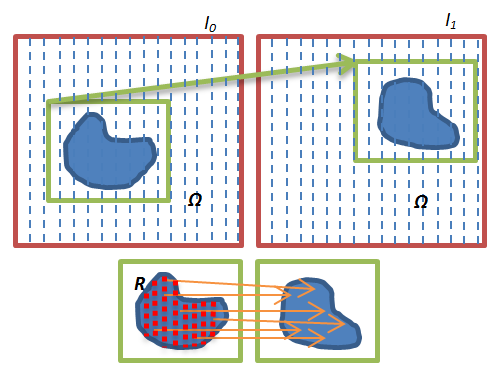
\includegraphics[width=1.0\textwidth]{../images/diagram.png}
    \end{column}
  \end{columns}
\end{frame}

\section{Object Flow}

\begin{frame}
	\frametitle{Pipeline}
  \begin{columns}[T]
    \begin{column}{.5\textwidth}
		\begin{block}{Object flow pipeline}
3 main steps: Tracking, Segmentation and Flow estimation.
What information to use to refine the object motion?	
		\end{block}
    \end{column}
    \begin{column}{.5\textwidth}
		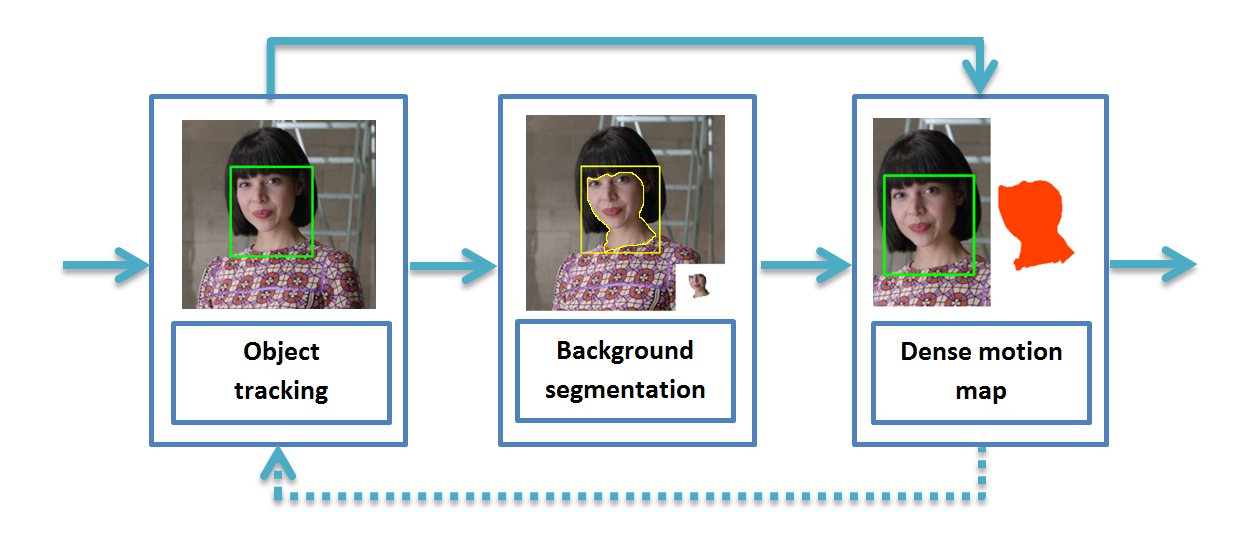
\includegraphics[width=1.0\textwidth]{../images/system.png}
    \end{column}
  \end{columns}
\end{frame}


\subsection{Tracking}

\begin{frame}
	\frametitle{Tracking}
  \begin{columns}[T]
    \begin{column}{.5\textwidth}
		\begin{block}{Tracking}
Tracking by detection methods have shown very good performance in 
modern benchmarks.
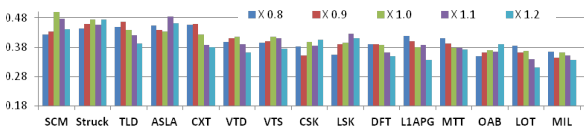
\includegraphics[width=1.0\textwidth]{../images/trackers_performance.png}
 	
		\end{block}
    \end{column}
    \begin{column}{.5\textwidth}
		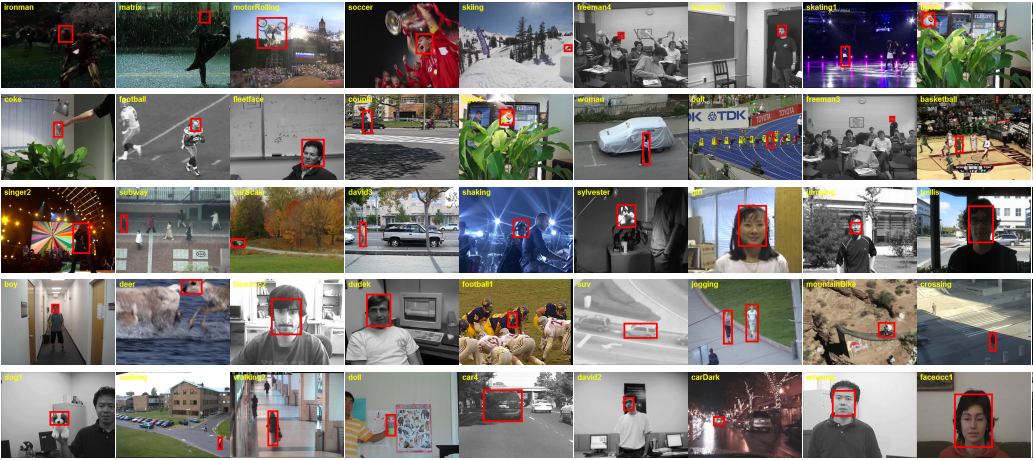
\includegraphics[width=1.0\textwidth]{../images/tr_db.png}
    \end{column}
  \end{columns}
\end{frame}

\subsection{Segmentation}

\begin{frame}
	\frametitle{Segmentation}
  \begin{columns}[T]
    \begin{column}{.33\textwidth}

Tracker window offers valuable information for object segmentation. Can it be completed naturally by video dynamics?		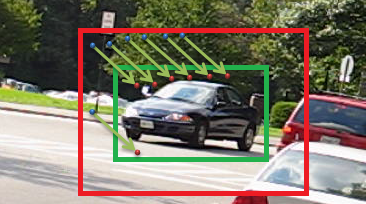
\includegraphics[width=1.0\textwidth]{../images/tracking_points.png}

    \end{column}	
    \begin{column}{.66\textwidth}
		\begin{block}{Background tracking} 
	Regions outside window can be labelled as background...	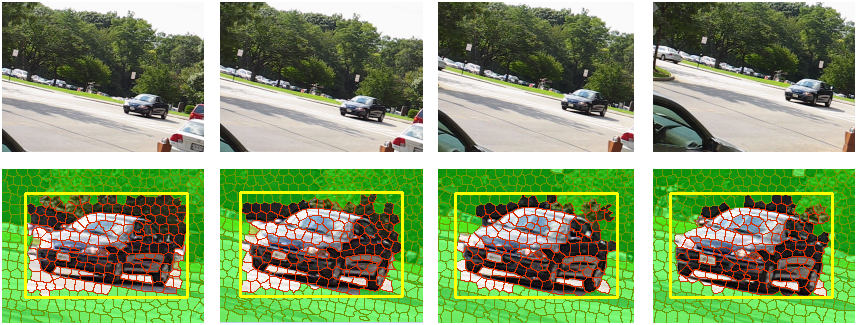
\includegraphics[width=1.0\textwidth]{../images/suppixflow2.png}
		\end{block}
    \end{column}	
    
  \end{columns}  
\end{frame}


\subsection{Background tracking}

\begin{frame}[shrink=15]
	\frametitle{Segmentation}
  \begin{columns}[T]
    \begin{column}{.5\textwidth}
		\begin{block}{Superpixel flow} 
A superpixel matching method is used to track background regions. 
This matching can be modelled with 
a pairwise Markov Random Field.

$ E(l) = \displaystyle \sum_{p \in \Gamma} D_p(l_p;I_0,I_1)+
\sum_{(p,q): q \in \mathcal{N}_r} S_{p,q}(l_p,l_q) $  

With $l$ the set of labels of the superpixels in $I_0$,
that match with those in $I_1$. $\mathcal{N}_r$ is a neighbourhood of radius $r$ of the superpixel $p$. $\Gamma$ is the set of superpixels in an image.
 
	\end{block}
    \end{column}	
    \begin{column}{.5\textwidth}
    		\begin{block}{Data and Spatial terms} 
    		The correspondent superpixels are similar.
    $ D_p(l_p;I_0,I_1) = \sqrt{ 1 - \frac{1}{\sqrt{\bar{ \boldsymbol{h} }(p) \bar{ \boldsymbol{h} }(p')N^2} } \sum_{i}\sqrt{ \boldsymbol{h}_{i}(p) \boldsymbol{h}_{i}(p')} }. $
Similar superpixels in one frame have similar motion vector.
$ S_{p,q}(l_p, l_q) = \lambda(p)
  \sqrt{\frac{|u_{p_c}-u_{q_c}|}{\|p_c-q_c\|}+ \frac{|v_{p_c}-v_{q_c}|}{\|p_c-q_c\|}} $    
    		\end{block}
    \end{column}	
  \end{columns}  
\end{frame}

\subsection{Segmentation refinement}

\begin{frame}
	\frametitle{Segmentation}
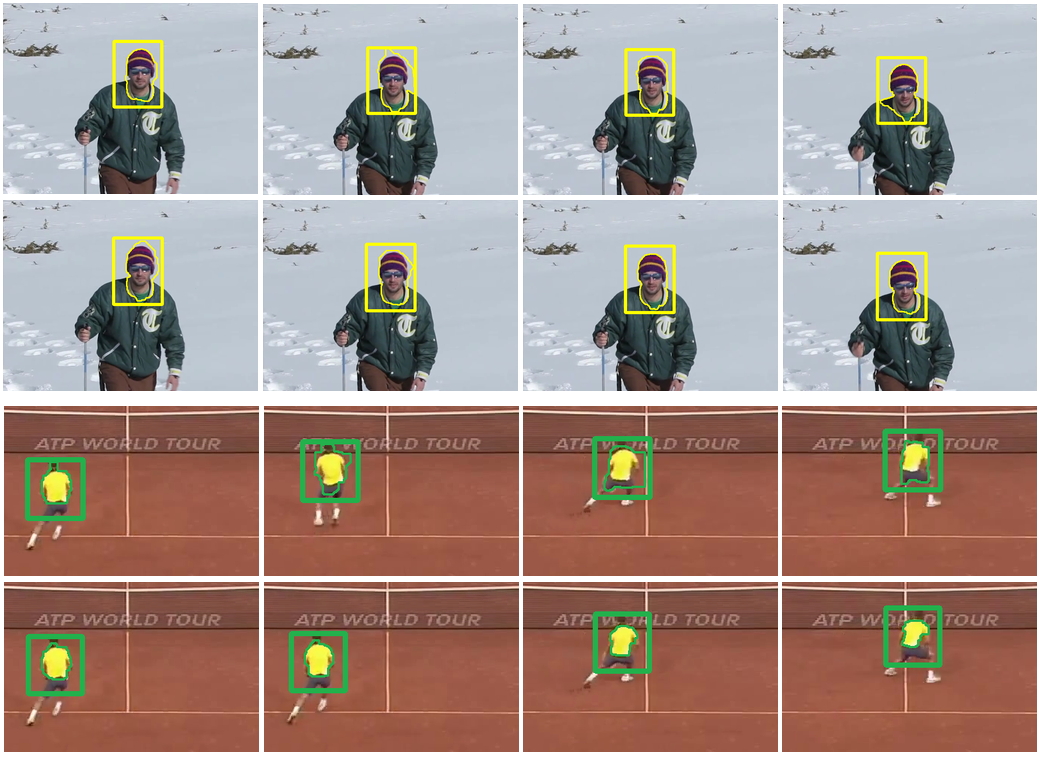
\includegraphics[height=0.85\textheight]{../images/compareSegm2.png}
\end{frame}

\subsection{More results}

\begin{frame}
	\frametitle{Segmentation}
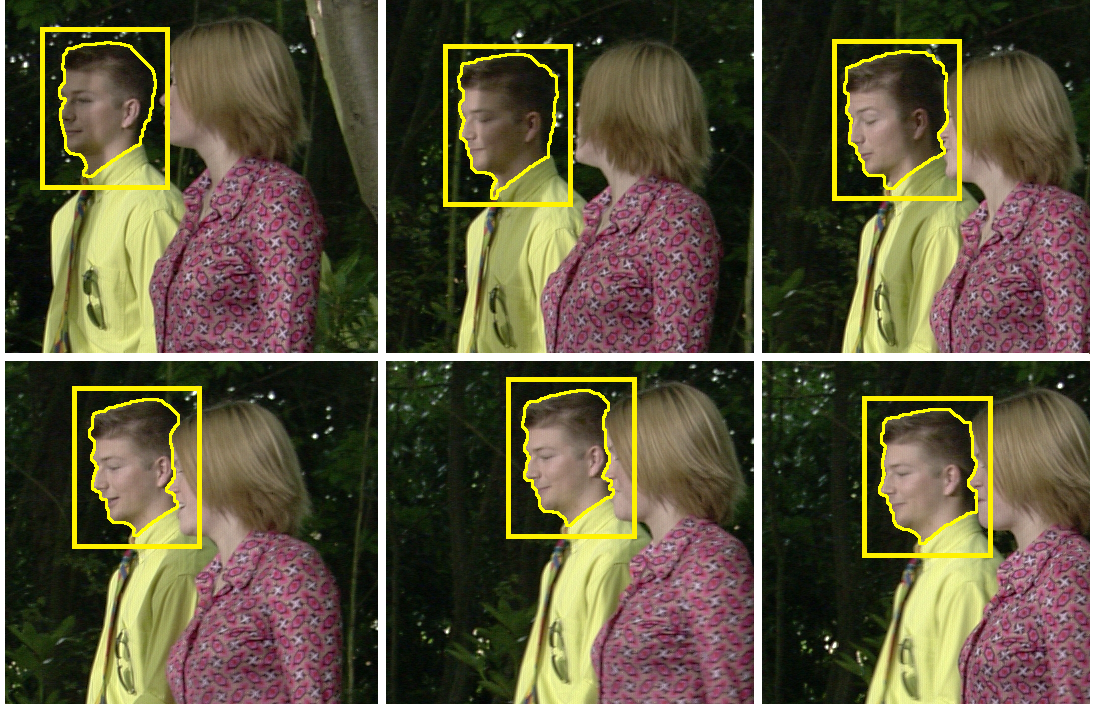
\includegraphics[width=1.00\textwidth]{../images/Sequence2.png}
\end{frame}

\subsection{Flow estimation}

\begin{frame}
	\frametitle{Flow estimation}
	In which parts of an image is valid the optical flow smoothness prior?
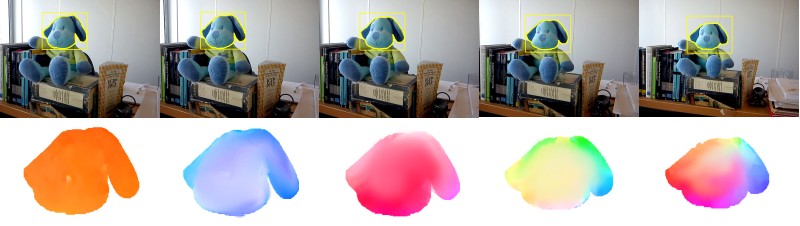
\includegraphics[width=1.00\textwidth]{../images/objectflow.png}
\end{frame}

\section{Results}

\subsection{Visual}

\begin{frame}
	\frametitle{Visual results}
	Extrapolation results between frame 2 distant frames by using 
	integrated flow.
	GT Object. Object flow backward, Object flow forward, Optical flow backward, and forward. Simple Flow.
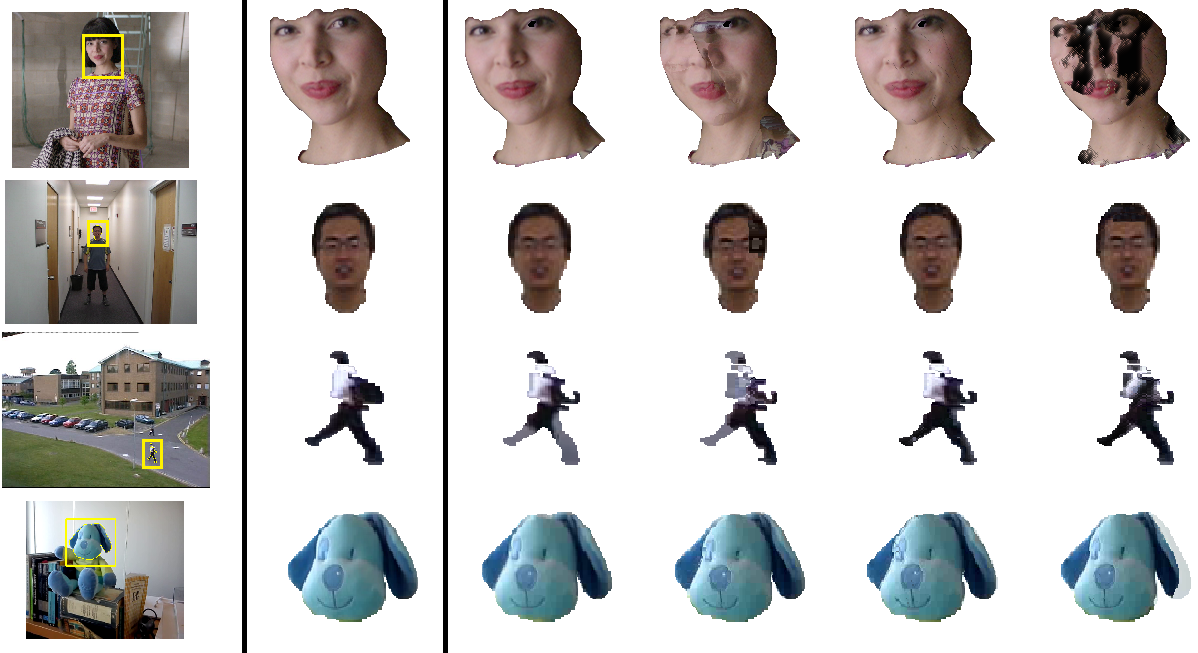
\includegraphics[height=0.5\textheight]{../images/extrapolated.png}
\end{frame}

\subsection{Numerical}

\begin{frame}
	\frametitle{Numerical results}
	PSNR for every extrapolated frame.
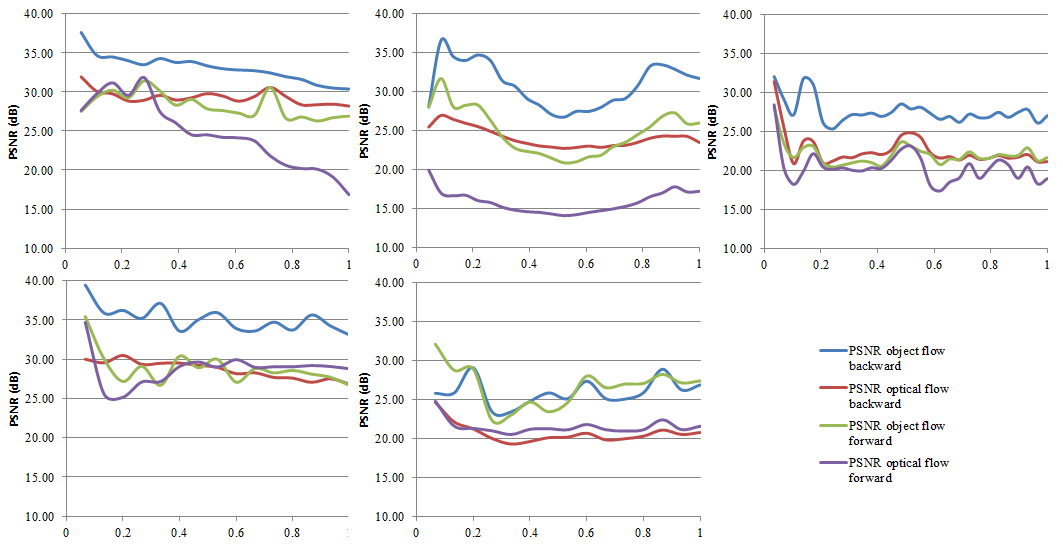
\includegraphics[width=1.0\textwidth]{../images/psnr.png}
\end{frame}

\begin{frame}
	\frametitle{Numerical results}
	Comparing several optical flow method with the object flow.
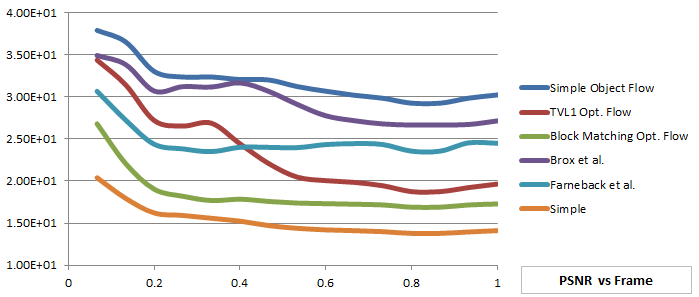
\includegraphics[width=1.0\textwidth]{../images/psnr2.png}
\end{frame}

\section{Applications}

\subsection{Video edition}

\begin{frame}
	\frametitle{Video edition}
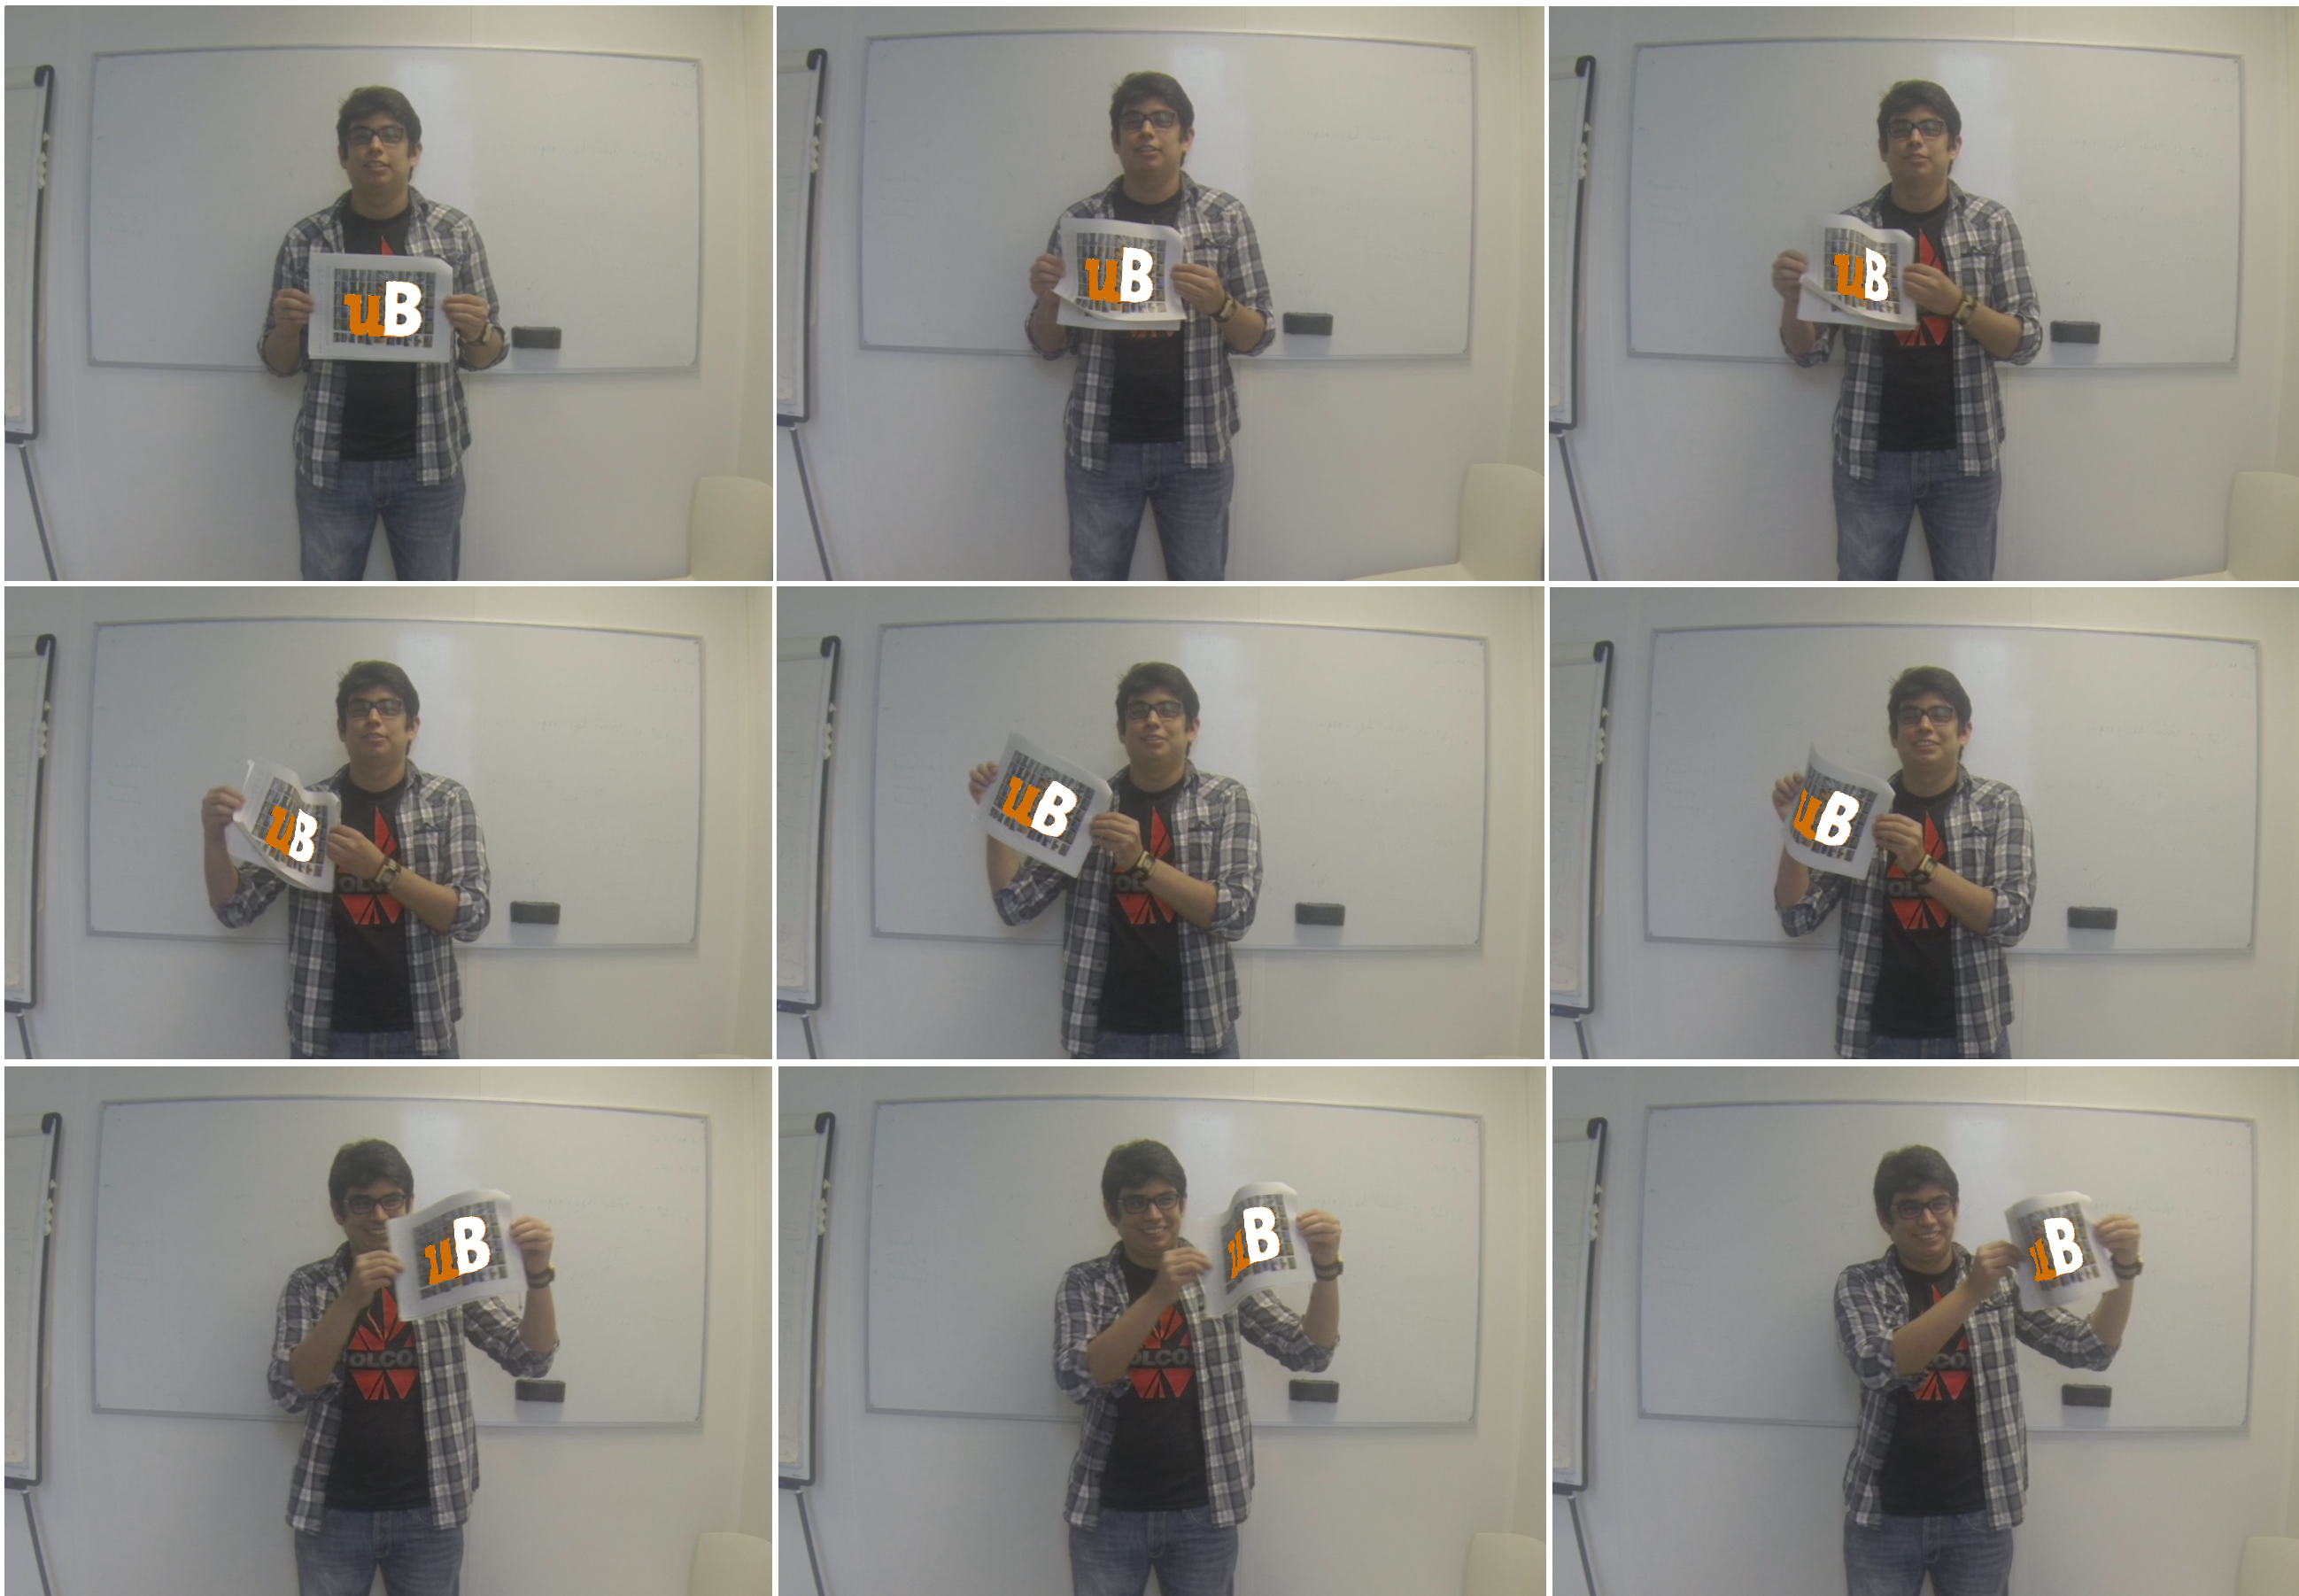
\includegraphics[width=1.0\textwidth]{../images/longUB.png}
\end{frame}

\subsection{Structure from Motion}

\begin{frame}
	\frametitle{SfM}
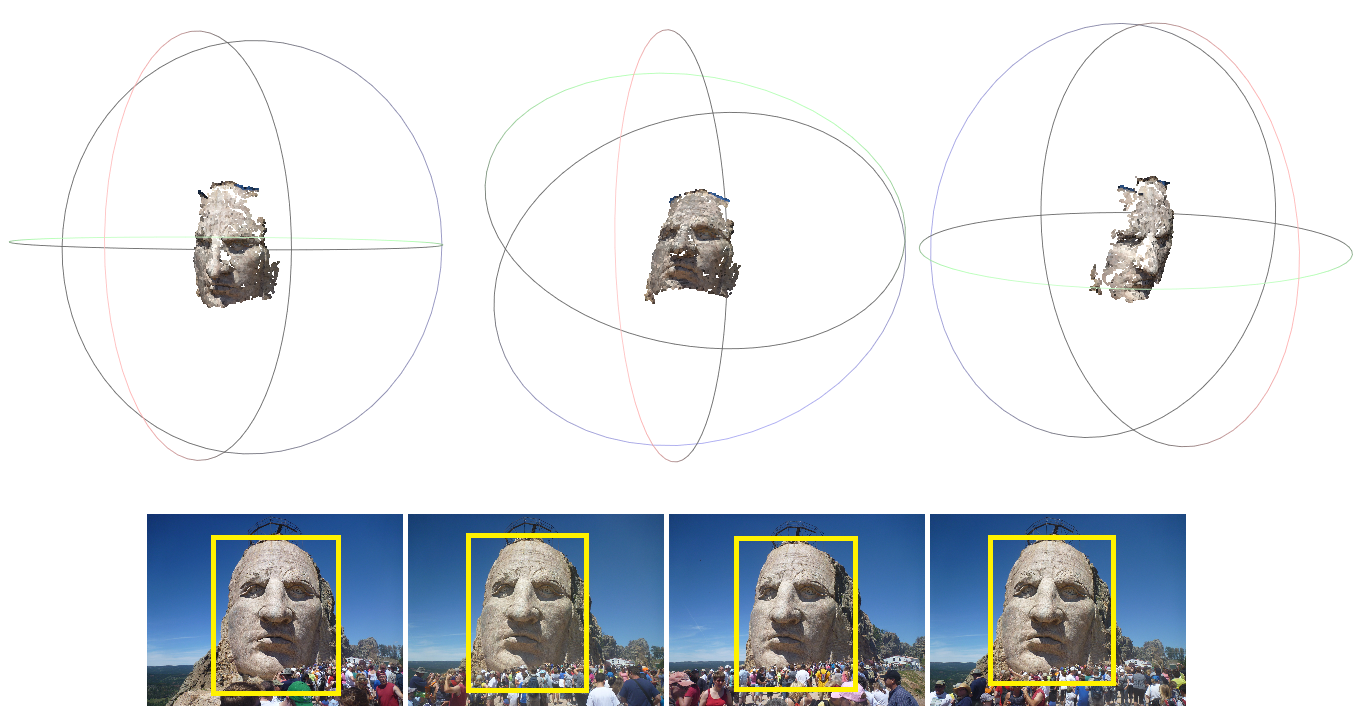
\includegraphics[width=1.0\textwidth]{../images/SFM.png}
\end{frame}

\section{Conclusions}

\begin{frame}
\frametitle{Conclusions}
\begin{enumerate}
\item The object flow problem is presented.
\item A method to match superpixel is explored.
\item An algorithm for object segmentation in video is explained.
\item A system to compute the object flow is proposed.
\item This system has shown to be more precise for dense object motion estimation than regular optical flow methods. 
\item Examples of the use of the 
object flow in real scenarios are presented.
\end{enumerate}

\end{frame}


\end{document}